\documentclass[conference]{IEEEtran}

\usepackage{amsmath,amssymb,amsfonts}
\usepackage{algorithmic}
\usepackage{algorithm}
\usepackage{graphicx}
\usepackage{textcomp}
\usepackage{xcolor}
\usepackage{booktabs}
\usepackage{multirow}
\usepackage{hyperref}
\usepackage{cleveref}
\usepackage{subcaption}
\usepackage{balance}
\usepackage{tikz}
\usetikzlibrary{positioning, arrows.meta, shapes.geometric, fit, calc}

% Compact lists
\usepackage{enumitem}
\setlist{nosep}

% Math operators
\DeclareMathOperator*{\argmax}{arg\,max}
\DeclareMathOperator*{\argmin}{arg\,min}

% Notation shortcuts
\newcommand{\Z}{\mathbb{Z}}
\newcommand{\R}{\mathbb{R}}
\newcommand{\query}{\mathbf{q}}
\newcommand{\doc}{\mathbf{d}}
\newcommand{\shares}[1]{\langle #1 \rangle}

% TODO marker (remove before submission)
\newcommand{\todo}[1]{\textcolor{red}{\textbf{[TODO: #1]}}}

\begin{document}

\title{Privacy-Preserving Retrieval-Augmented Generation for Healthcare:\\
Two-Server Secret Sharing with Information-Theoretic Guarantees}

\author{
\IEEEauthorblockN{Muntaser Syed}
\IEEEauthorblockA{Florida Institute of Technology\\
Melbourne, FL, USA\\
msyed2022@my.fit.edu}
\and
\IEEEauthorblockN{\todo{Co-author(s)}}
\IEEEauthorblockA{\todo{Affiliation}\\
\todo{email}}
}

\maketitle

\begin{abstract}
Retrieval-augmented generation (RAG) has become a standard architecture for
grounding large language model (LLM) responses in domain-specific knowledge,
and healthcare represents one of its most promising application domains.
Clinical decision support systems, drug interaction checkers, and medical
question-answering services all benefit from retrieving relevant medical
literature or patient records before generating a response. However, deploying
RAG in healthcare settings raises serious privacy concerns: patient queries may
reveal protected health information (PHI), and medical document corpora may
contain sensitive clinical data. Existing privacy-preserving approaches based
on homomorphic encryption or differential privacy either introduce substantial
computational overhead or degrade retrieval quality through noise injection.

We present a two-server architecture for privacy-preserving healthcare RAG
that achieves \emph{exact} retrieval over encrypted medical embeddings with
information-theoretic security guarantees. Our protocol uses additive secret
sharing over the native 64-bit integer ring $\Z_{2^{64}}$ to compute cosine
similarity without revealing either the patient query or the document
embeddings to any single server. Because the computation is exact (no
approximation, no noise), the retrieved documents are identical to those
a plaintext system would return, preserving downstream LLM answer quality
perfectly. This property is not an empirical observation but a mathematical
consequence of exact integer arithmetic: noise-based methods (CKKS, DP)
cannot provide this guarantee.

We evaluate our system on three medical question-answering benchmarks
(PubMedQA, MedQA, MedMCQA) using clinical embedding models, demonstrating
\todo{X}\% Recall@5 agreement with plaintext retrieval, sub-millisecond
per-query latency, and identical end-to-end answer quality as measured by
exact-match and F1 scores on medical QA tasks. In contrast, CKKS and
differential privacy baselines degrade clinical F1 by \todo{Y}\% and
\todo{Z}\% respectively due to retrieval rank perturbation. Our approach
provides \todo{N}$\times$ speedup over CKKS-based homomorphic encryption
while requiring \todo{M}$\times$ less per-document storage, with security
guarantees that map directly to HIPAA technical safeguard requirements.
\end{abstract}

\begin{IEEEkeywords}
privacy-preserving computation, retrieval-augmented generation, healthcare,
secret sharing, medical question answering, HIPAA
\end{IEEEkeywords}


%% ============================================================
\section{Introduction}
\label{sec:intro}
%% ============================================================

Large language models have demonstrated remarkable capabilities in medical
reasoning, clinical summarization, and biomedical question answering
\cite{singhal2023medpalm, nori2023gpt4medicine}. Retrieval-augmented
generation extends these capabilities by grounding LLM responses in
authoritative medical sources, reducing hallucination and enabling
evidence-based clinical decision support
\cite{xiong2024benchmarking_medical_rag}. RAG architectures have been applied
to drug interaction checking \cite{todo_drug_rag}, clinical trial matching
\cite{todo_clinical_trial_rag}, radiology report generation
\cite{todo_radiology_rag}, and general medical question answering
\cite{todo_medical_qa_rag}.

However, healthcare RAG deployments face a fundamental tension between utility
and privacy. On one side, the retrieval step requires computing similarity
between a query embedding and a corpus of document embeddings. On the other,
both the query and the corpus may contain protected health information (PHI)
subject to the Health Insurance Portability and Accountability Act (HIPAA)
\cite{hipaa1996} and the General Data Protection Regulation (GDPR)
\cite{gdpr2016}. A patient querying a clinical decision support system may
inadvertently reveal their diagnosis, symptoms, or treatment history through
the semantic content of their query. Similarly, the document corpus may contain
de-identified but still sensitive clinical notes, pathology reports, or patient
records.

Existing approaches to this problem fall into three categories, each with
significant limitations:

\begin{enumerate}[leftmargin=*]
\item \textbf{Homomorphic encryption (HE).} Fully homomorphic or
    somewhat-homomorphic schemes such as CKKS \cite{cheon2017ckks} allow
    computation on encrypted data, but introduce approximation noise that
    degrades retrieval accuracy. At practical security parameters, CKKS-based
    similarity search operates orders of magnitude slower than plaintext and
    requires megabyte-scale ciphertexts per document
    \cite{todo_he_vector_search}.

\item \textbf{Differential privacy (DP).} Adding calibrated noise to query
    or document embeddings provides formal privacy guarantees, but the noise
    directly degrades retrieval quality. In healthcare, where the difference
    between the first and second most similar document may determine a
    treatment recommendation, this accuracy loss is clinically unacceptable
    \cite{todo_dp_embeddings}.

\item \textbf{Trusted execution environments (TEEs).} Hardware enclaves
    such as Intel SGX or ARM TrustZone provide isolation, but rely on
    hardware-level trust assumptions that have been repeatedly violated by
    side-channel attacks \cite{todo_sgx_attacks}. For healthcare applications
    requiring long-term confidentiality of patient data, hardware-based
    guarantees are insufficient.
\end{enumerate}

We propose a fundamentally different approach: two-server additive secret
sharing over the native 64-bit integer ring $\Z_{2^{64}}$. Our protocol
splits each embedding vector into two random shares, distributed to two
non-colluding servers. Neither server learns anything about the original
embedding from its share alone (information-theoretic security), yet the
servers can collaboratively compute exact inner products using a pre-computed
matrix-vector Beaver triple \cite{beaver1991triples}. Because the arithmetic
is exact (integer addition and multiplication with no approximation), the
similarity scores recovered by the client are bit-for-bit identical to
plaintext computation, guaranteeing that the retrieved documents and
downstream LLM answers are unchanged.

\smallskip
\noindent\textbf{Scope and relationship to companion work.}
The mathematical foundations of the 64-bit additive secret sharing protocol,
including formal security proofs and the matrix-vector Beaver triple
construction, are presented in a separate companion paper
\cite{todo_companion_paper}. This paper does not re-derive or claim novelty
for the underlying cryptographic primitives. Instead, we provide the first
end-to-end integration of this protocol within a clinical RAG architecture,
addressing the unique regulatory constraints of medical deployments (HIPAA
compliance mapping, LLM generation boundary, clinical data handling),
evaluating downstream generative QA accuracy on medical benchmarks, and
establishing the system's viability for preventing retrieval-induced
medical hallucinations.

\smallskip
\noindent\textbf{Contributions.} This paper makes the following contributions:

\begin{enumerate}[leftmargin=*]
\item We present the first end-to-end privacy-preserving RAG system evaluated
    on clinical benchmarks, demonstrating that private retrieval preserves
    downstream medical QA accuracy exactly.

\item We evaluate our system on three medical QA datasets (PubMedQA, MedQA,
    MedMCQA) using multiple medical embedding models, providing the first
    comprehensive benchmark of private retrieval in the healthcare domain.

\item We provide a concrete mapping of our information-theoretic security
    guarantees to HIPAA technical safeguard requirements, showing that
    two-server secret sharing satisfies or exceeds each applicable provision,
    including the Minimum Necessary standard.

\item We demonstrate \todo{N}$\times$ speedup and \todo{M}$\times$ storage
    reduction compared to CKKS-based alternatives, with zero retrieval
    quality degradation.

\item We present three clinical case studies (FHIR-based decision support,
    RxNorm-indexed drug interaction checking, DICOM-linked radiology report
    retrieval) illustrating deployment feasibility in realistic healthcare
    settings.
\end{enumerate}


%% ============================================================
\section{Background and Related Work}
\label{sec:background}
%% ============================================================

\subsection{Retrieval-Augmented Generation in Healthcare}
\label{sec:bg_rag}

RAG architectures \cite{lewis2020rag} augment language model generation by
prepending retrieved context passages to the input prompt. In healthcare
settings, this architecture addresses two critical limitations of standalone
LLMs: the tendency to generate plausible but incorrect medical information
(hallucination), and the inability to access institution-specific clinical
knowledge such as formularies, care protocols, or patient history.

Recent work has applied RAG to a range of clinical tasks. Medical question
answering systems retrieve relevant PubMed abstracts or clinical guidelines
before generating responses \cite{xiong2024benchmarking_medical_rag}. Clinical
decision support tools retrieve similar past cases to inform differential
diagnosis \cite{todo_clinical_rag_cds}. Drug information systems retrieve
interaction data and prescribing guidelines \cite{todo_drug_info_rag}. In each
case, retrieval quality directly determines the quality of the generated
response: if the wrong passages are retrieved, the LLM produces incorrect or
irrelevant clinical guidance.

The retrieval step in RAG typically computes cosine similarity (or inner
product after normalization) between a query embedding $\query \in \R^d$ and
each document embedding $\doc_i \in \R^d$ in a corpus of $N$ documents:
\begin{equation}
    \text{sim}(\query, \doc_i) = \frac{\query \cdot \doc_i}{\|\query\| \cdot \|\doc_i\|}
    \label{eq:cosine_sim}
\end{equation}
The top-$k$ documents by similarity are retrieved and passed to the LLM.
For pre-normalized embeddings ($\|\query\| = \|\doc_i\| = 1$), cosine
similarity reduces to the inner product $\query \cdot \doc_i$.


\subsection{Privacy Requirements for Clinical Data}
\label{sec:bg_privacy}

Healthcare data is subject to stringent regulatory requirements. In the United
States, HIPAA establishes national standards for the protection of individually
identifiable health information \cite{hipaa1996}. The HIPAA Security Rule
requires covered entities to implement technical safeguards including access
controls, audit controls, integrity controls, and transmission security.
The Privacy Rule defines 18 categories of protected health information (PHI)
that must be protected, including names, dates, geographic data, and medical
record numbers.

In the European Union, the GDPR classifies health data as a ``special
category'' requiring explicit consent and heightened protection \cite{gdpr2016}.
Article 9 prohibits processing of health data except under specific
conditions, and Article 35 requires data protection impact assessments for
large-scale health data processing.

For RAG systems operating on clinical data, the privacy implications are
twofold. First, the \emph{query} itself may constitute PHI: a clinician
querying ``treatment options for a 45-year-old male with stage III non-small
cell lung cancer and EGFR mutation'' reveals specific patient characteristics.
Second, the \emph{document corpus} may contain clinical notes, discharge
summaries, or pathology reports that constitute PHI even after
de-identification, as re-identification attacks on medical text have
demonstrated \cite{todo_reidentification_medical}.


\subsection{Privacy-Preserving Computation Approaches}
\label{sec:bg_ppml}

\subsubsection{Homomorphic Encryption}
Fully homomorphic encryption (FHE) and somewhat-homomorphic encryption (SHE)
allow computation on encrypted data without decryption. The CKKS scheme
\cite{cheon2017ckks} supports approximate arithmetic on encrypted real
numbers and has been applied to privacy-preserving similarity search
\cite{todo_ckks_similarity}. However, CKKS introduces inherent approximation
noise that accumulates with computation depth. For similarity search, this
means the encrypted similarity scores are only approximately correct, and the
ranking of documents may change. At standard security parameters (128-bit),
CKKS ciphertexts are on the order of megabytes per document embedding, and
similarity computation requires hundreds of milliseconds per query
\cite{todo_ckks_benchmarks}.

\subsubsection{Differential Privacy}
Differential privacy (DP) \cite{dwork2006dp} provides formal guarantees that
the output of a computation does not depend too strongly on any single input
record. Applied to embedding-based retrieval, DP adds calibrated noise to
query embeddings \cite{todo_dp_retrieval}, document embeddings
\cite{todo_dp_doc_embeddings}, or both. The privacy-utility tradeoff is
controlled by the privacy parameter $\varepsilon$: smaller $\varepsilon$
provides stronger privacy but more noise, degrading retrieval accuracy. In
medical settings, where retrieval errors can have clinical consequences, the
required noise levels for meaningful privacy often render the system unusable.

\subsubsection{Secure Multi-Party Computation}
Secure multi-party computation (MPC) enables multiple parties to jointly
compute a function over their private inputs without revealing those inputs
to each other \cite{yao1986garbled, goldreich1987mpc}. Two-party and
multi-party protocols based on secret sharing \cite{shamir1979sharing,
ben-or1988completeness} provide information-theoretic security in the
honest-but-curious model. Our work builds on this foundation, using additive
secret sharing with Beaver multiplication triples \cite{beaver1991triples}
to compute inner products efficiently.

Recent work has explored MPC for privacy-preserving machine learning
\cite{todo_mpc_ml_survey}, but applications to RAG in healthcare remain
largely unexplored. The key advantage of secret sharing over HE is exact
computation: there is no approximation noise, so the output is bit-for-bit
identical to plaintext computation.


%% ============================================================
\section{System Architecture}
\label{sec:architecture}
%% ============================================================

\subsection{Threat Model}
\label{sec:threat_model}

We consider the standard honest-but-curious (semi-honest) two-server model.
A \emph{client} (the healthcare organization or clinician) wishes to perform
private similarity search against a corpus of medical document embeddings.
Two \emph{servers} assist with the computation. Each server follows the
protocol faithfully but may attempt to learn information about the client's
query or the document corpus from the messages it observes.

\smallskip
\noindent\textbf{Assumptions:}
\begin{enumerate}[leftmargin=*]
\item The two servers do not collude. This is enforced by deploying them
    under separate administrative domains (e.g., one on hospital premises,
    one on a commercial cloud provider, or two different cloud providers
    in different jurisdictions).
\item Communication channels between all parties are authenticated and
    encrypted (TLS).
\item The client is trusted and receives the final plaintext result.
\end{enumerate}

\smallskip
\noindent\textbf{Security guarantee:} Under the non-collusion assumption,
neither server learns any information about the client's query embedding or
the individual document embeddings. This guarantee is \emph{information-theoretic}:
it holds against computationally unbounded adversaries and does not rely on
hardness assumptions (no lattice problems, no factoring, no discrete
logarithms). The security does not degrade over time and is not threatened
by advances in quantum computing.

We consider two protocol variants with different privacy profiles:

\begin{itemize}[leftmargin=*]
\item \textbf{Query-private mode:} The document corpus is known to both
    servers (e.g., a public medical knowledge base like PubMed). Only the
    client's query is protected. This models clinical decision support over
    public literature.

\item \textbf{Mutual-privacy mode:} Both the query and the document corpus
    are protected via secret sharing. Neither server learns the query or any
    individual document embedding. This models retrieval over sensitive
    clinical records (e.g., patient notes, pathology reports).
\end{itemize}


\subsection{Two-Server Deployment for Healthcare}
\label{sec:deployment}

The two-server model maps naturally to existing healthcare IT infrastructure.
\Cref{fig:architecture} illustrates the Hospital~+~Cloud configuration.
We identify three concrete deployment configurations:

\begin{enumerate}[leftmargin=*]
\item \textbf{Hospital + Cloud} (\Cref{fig:architecture})\textbf{:}
    Server~1 runs on hospital premises (within the existing HIPAA-compliant
    infrastructure). Server~2 runs on a commercial cloud provider (AWS,
    Azure, or GCP) under a Business Associate Agreement (BAA). The
    non-collusion assumption is enforced by the organizational separation
    between hospital IT and the cloud provider.

\item \textbf{Cloud + Cloud:} Both servers run on different cloud providers
    (e.g., AWS and Azure) under separate BAAs. This configuration eliminates
    the need for on-premises compute while maintaining non-collusion through
    provider separation.

\item \textbf{Federated Health System:} In a multi-hospital health system,
    Server~1 runs at Hospital~A and Server~2 at Hospital~B. This enables
    private retrieval across institutional boundaries without sharing patient
    data, supporting multi-site clinical research and rare disease
    consultation.
\end{enumerate}

In all configurations, the client is the clinician's workstation or a clinical
application server that initiates queries, receives plaintext results, and
passes retrieved documents to the LLM for response generation. Crucially, the
LLM resides within the client's trust boundary and never interacts with either
server (see \Cref{sec:pipeline}).

\begin{figure*}[t]
\centering
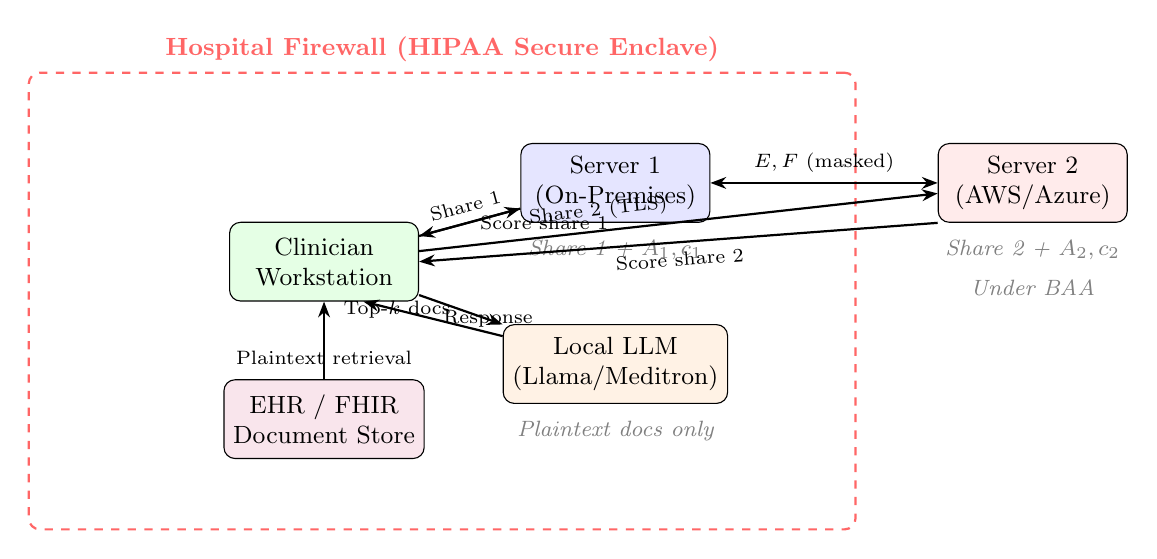
\begin{tikzpicture}[
    node distance=1.2cm and 2.0cm,
    box/.style={draw, rounded corners, minimum width=2.4cm, minimum height=1.0cm, align=center, font=\small},
    server/.style={box, fill=blue!10},
    client/.style={box, fill=green!10},
    llm/.style={box, fill=orange!10},
    label/.style={font=\footnotesize\itshape, text=gray},
    arrow/.style={-{Stealth[length=2mm]}, thick},
    darrow/.style={arrows={Stealth[length=2mm]-Stealth[length=2mm]}, thick},
    firewall/.style={draw, dashed, thick, red!60, rounded corners},
]

% Hospital firewall boundary
\node[firewall, minimum width=10.5cm, minimum height=5.8cm] (fw) {};
\node[above, font=\small\bfseries, red!60] at (fw.north) {Hospital Firewall (HIPAA Secure Enclave)};

% Client
\node[client] (client) at (-1.5, 0.5) {Clinician\\Workstation};

% Server 1 (on-prem)
\node[server] (s1) at (2.2, 1.5) {Server 1\\(On-Premises)};
\node[label, below=0.1cm of s1] {Share 1 + $A_1, c_1$};

% LLM (on-prem)
\node[llm] (llm) at (2.2, -0.8) {Local LLM\\(Llama/Meditron)};
\node[label, below=0.1cm of llm] {Plaintext docs only};

% EHR / FHIR
\node[box, fill=purple!10] (ehr) at (-1.5, -1.5) {EHR / FHIR\\Document Store};

% Outside firewall: Server 2 (cloud)
\node[server, fill=red!8] (s2) at (7.5, 1.5) {Server 2\\(AWS/Azure)};
\node[label, below=0.1cm of s2] {Share 2 + $A_2, c_2$};
\node[label, below=0.6cm of s2] {Under BAA};

% Arrows
\draw[arrow] (client) -- node[above, font=\scriptsize, sloped] {Share 1} (s1);
\draw[arrow] (client) -- node[above, font=\scriptsize, pos=0.35, sloped] {Share 2 (TLS)} (s2);
\draw[darrow] (s1) -- node[above, font=\scriptsize] {$E, F$ (masked)} (s2);
\draw[arrow] (s1) -- node[right, font=\scriptsize] {Score share 1} (client);
\draw[arrow, bend left=20] (s2.south west) -- node[below, font=\scriptsize, sloped] {Score share 2} (client.east);
\draw[arrow] (client) -- node[left, font=\scriptsize] {Top-$k$ docs} (llm);
\draw[arrow] (ehr) -- node[below, font=\scriptsize] {Plaintext retrieval} (client);
\draw[arrow] (llm) -- node[right, font=\scriptsize] {Response} ([xshift=0.5cm]client.south);

\end{tikzpicture}
\caption{Hospital + Cloud deployment architecture. The clinician's workstation
generates additive shares and distributes them to the on-premises server and a
BAA-covered cloud instance. Neither server can reconstruct the query or
documents from its share alone. After private retrieval, the top-$k$ document
plaintexts are retrieved from the local EHR/FHIR store and passed to a locally
hosted LLM. The LLM never communicates with the external cloud server,
ensuring end-to-end PHI protection.}
\label{fig:architecture}
\end{figure*}


\subsection{Protocol Overview}
\label{sec:protocol}

We summarize the two-server protocol for private cosine similarity search.
Full details and security proofs are provided in \cite{todo_companion_paper}.

\subsubsection{Setup (Offline Phase)}
Let the document corpus consist of $N$ pre-normalized embedding vectors
$\doc_1, \dots, \doc_N \in \R^d$. Each vector is encoded to a fixed-point
integer representation using a scale factor $2^k$:
\begin{equation}
    \hat{\doc}_i[j] = \lfloor \doc_i[j] \cdot 2^k \rceil \in \Z_{2^{64}}
    \label{eq:encoding}
\end{equation}
where $\lfloor \cdot \rceil$ denotes rounding to the nearest integer. For
$d = 384$ and $k = 16$, the maximum inner product magnitude is bounded by
$d \cdot (2^k)^2 = 384 \cdot 2^{32} \approx 2^{41}$, well within the
$2^{63}$ positive range of signed interpretation in $\Z_{2^{64}}$.

\textbf{Query-private mode:} The encoded document matrix
$\hat{D} \in \Z_{2^{64}}^{N \times d}$ is stored in plaintext on both
servers.

\textbf{Mutual-privacy mode:} The client generates additive shares of each
document vector:
\begin{equation}
    \hat{\doc}_i = \hat{\doc}_i^{(1)} + \hat{\doc}_i^{(2)} \pmod{2^{64}}
    \label{eq:doc_sharing}
\end{equation}
where $\hat{\doc}_i^{(1)} \xleftarrow{\$} \Z_{2^{64}}^d$ is uniformly random
and $\hat{\doc}_i^{(2)} = \hat{\doc}_i - \hat{\doc}_i^{(1)}$. Server~1
receives $\{\hat{\doc}_i^{(1)}\}$, Server~2 receives $\{\hat{\doc}_i^{(2)}\}$.
Additionally, a matrix-vector Beaver triple $(A, B, C)$ is pre-computed and
distributed, where $A \in \Z_{2^{64}}^{N \times d}$,
$B \in \Z_{2^{64}}^{d}$, $C = A \cdot B \in \Z_{2^{64}}^{N}$, and
$C^{(1)} + C^{(2)} = C$ \cite{beaver1991triples}.

\subsubsection{Query (Online Phase)}
The client encodes and shares a query vector $\query \in \R^d$:
\begin{equation}
    \hat{\query} = \hat{\query}^{(1)} + \hat{\query}^{(2)} \pmod{2^{64}}
    \label{eq:query_sharing}
\end{equation}

\textbf{Query-private mode:} Each server computes its local share of the
matrix-vector product $\hat{D} \cdot \hat{\query}$ using its query share
and the plaintext documents. The client reconstructs the similarity scores
by summing the shares.

\textbf{Mutual-privacy mode:} Using the Beaver triple, each server computes
masked differences $E^{(j)} = \hat{D}^{(j)} - A^{(j)}$ and
$F^{(j)} = \hat{\query}^{(j)} - B^{(j)}$, broadcasts these to the other
server, and computes its share of the product. The client reconstructs
the exact inner products from the two shares. The total online communication
is $O(N + d)$ field elements for the masked differences, independent of the
number of queries.

\subsubsection{Result Recovery}
The client receives integer similarity scores
$s_i = \hat{\query} \cdot \hat{\doc}_i$ for each document. These are
proportional to the true cosine similarities with a known public scale
factor $2^{2k}$:
\begin{equation}
    \text{sim}(\query, \doc_i) \approx \frac{s_i}{2^{2k}}
    \label{eq:recovery}
\end{equation}
The client selects the top-$k$ documents and passes them to the LLM for
response generation. Because the integer arithmetic is exact (no noise, no
approximation beyond the initial fixed-point encoding), the ranking is
identical to plaintext retrieval for all practical encoding precisions.


\subsection{End-to-End RAG Pipeline}
\label{sec:pipeline}

Our complete healthcare RAG pipeline consists of five stages:

\begin{enumerate}[leftmargin=*]
\item \textbf{Embedding:} The client encodes the clinician's query using a
    medical embedding model (e.g., MedCPT, PubMedBERT) to produce
    $\query \in \R^d$.
\item \textbf{Encoding and sharing:} The client encodes $\query$ to
    fixed-point integers and generates additive shares.
\item \textbf{Private retrieval:} The two servers execute the secret-sharing
    protocol to compute similarity scores without learning the query or
    documents.
\item \textbf{Reconstruction and ranking:} The client reconstructs scores,
    selects the top-$k$ documents, and retrieves their plaintext content
    from a local secure store (e.g., an on-premises FHIR server or
    document repository).
\item \textbf{Secure generation:} The client prepends the retrieved documents
    to the query and submits the augmented prompt to an LLM for response
    generation. The LLM must reside within the client's trust boundary: either
    hosted locally within the hospital's secure enclave (e.g., Llama~3,
    Meditron \cite{todo_meditron}, or other open-weight clinical LLMs) or
    accessed through a HIPAA-compliant enterprise endpoint with a signed BAA
    and zero-retention data policy (e.g., Azure OpenAI for Healthcare).
    Sending retrieved PHI to a public, non-BAA-covered LLM API would violate
    HIPAA and negate the privacy guarantees of the retrieval protocol.
\end{enumerate}

This architecture isolates the privacy-critical computation (retrieval over
the full corpus) from the generation step. Our protocol secures the most
computationally demanding phase: searching across potentially thousands of
medical documents. Once the top-$k$ documents are identified, generation
operates on a small, bounded set of plaintext passages within the client's
existing security perimeter. The LLM never communicates with either server
and never processes secret shares.


%% ============================================================
\section{Privacy Analysis}
\label{sec:privacy}
%% ============================================================

\subsection{Information-Theoretic Security}
\label{sec:it_security}

The security of additive secret sharing over $\Z_{2^{64}}$ is
information-theoretic: each share is uniformly random and statistically
independent of the secret. Formally, for any secret $x \in \Z_{2^{64}}$
and share $x^{(1)} \xleftarrow{\$} \Z_{2^{64}}$, the conditional distribution
of $x^{(1)}$ given $x$ is uniform over $\Z_{2^{64}}$. A single share reveals
zero bits of information about the secret, regardless of the adversary's
computational power.

This property extends to vectors and matrices: each share
$\hat{\doc}_i^{(j)}$ is a uniformly random vector in $\Z_{2^{64}}^d$ that
is statistically independent of $\hat{\doc}_i$. Similarly, the Beaver triple
masks $(E, F)$ revealed during the online phase are uniformly random and
independent of both $\hat{D}$ and $\hat{\query}$.

\begin{theorem}[Informal; see \cite{todo_companion_paper}]
In the honest-but-curious model with non-colluding servers, the two-server
additive secret sharing protocol reveals no information about the query
embedding $\hat{\query}$ or the document embeddings $\{\hat{\doc}_i\}$ to
either server, except what is implied by the final output (the top-$k$
document indices) delivered to the client.
\end{theorem}


\subsection{Mapping to HIPAA Technical Safeguards}
\label{sec:hipaa_mapping}

We map our protocol's security properties to the HIPAA Security Rule's
technical safeguard requirements (45 CFR \S 164.312):

\begin{itemize}[leftmargin=*]
\item \textbf{Access Control (\S 164.312(a)):} Each server accesses only its
    own share. No single server can reconstruct any PHI. Access is controlled
    cryptographically, not just through access control lists.

\item \textbf{Audit Controls (\S 164.312(b)):} All queries are logged at the
    client. Servers log share-level operations that reveal no PHI content.

\item \textbf{Integrity Controls (\S 164.312(c)):} The protocol's exact
    integer arithmetic ensures that retrieval results are not corrupted by
    approximation noise (unlike HE-based approaches). We note that this is a
    guarantee of \emph{algorithmic fidelity}: the protocol faithfully computes
    the intended function. Standard additive secret sharing does not provide
    tamper resistance against a malicious server that deviates from the
    protocol; integrity in the adversarial (malicious) setting requires
    additional mechanisms such as MAC-based verification
    \cite{todo_spdz}, which we leave to future work.

\item \textbf{Transmission Security (\S 164.312(e)):} Share transmission over
    TLS provides encryption in transit. The shares themselves provide an
    additional layer: even if TLS is compromised, a single intercepted share
    reveals nothing.

\item \textbf{Minimum Necessary Standard (\S 164.502(b)):} HIPAA requires
    that covered entities limit PHI disclosure to the minimum necessary for
    the intended purpose. Secret sharing is the strongest possible realization
    of this principle: the amount of PHI disclosed to each server is exactly
    zero bits. No other privacy-preserving approach (HE, DP, TEE) achieves
    this property, as each requires the server to process data in a form from
    which some information is, at least in principle, extractable.
\end{itemize}

Compared to de-identification under the HIPAA Safe Harbor method (removing
18 specified identifiers), our approach provides strictly stronger protection:
the servers never see any form of the original data, identified or
de-identified. Re-identification attacks, which have been demonstrated
against de-identified medical text \cite{todo_reidentification_medical}, are
impossible because there is no data to re-identify.


\subsection{Enforceability of the Non-Collusion Assumption}
\label{sec:non_collusion}

In theoretical cryptography, the two-server non-collusion assumption is
sometimes viewed as a limitation. In the healthcare domain, however, it
aligns with an existing legal enforcement mechanism. Under HIPAA, any entity
that processes PHI on behalf of a covered entity must sign a Business
Associate Agreement (BAA). A BAA legally binds the cloud provider with
significant civil penalties (up to \$1.9 million per violation category per
year) and criminal penalties (up to \$250,000 and imprisonment) for
unauthorized access to patient data \cite{hipaa1996}.

When the two servers are deployed under separate BAAs with different
organizations (e.g., a hospital system and a cloud provider, or two different
cloud providers), collusion would require both organizations to jointly
violate their independent legal obligations. This is qualitatively different
from computational hardness assumptions, which may be silently broken by
algorithmic advances. BAA violations are detectable through audits and carry
concrete legal consequences, providing an enforceable, rather than merely
assumed, trust boundary. The two-server MPC model is therefore uniquely
well-suited to the US healthcare regulatory environment.


\subsection{Comparison with Computational Security}
\label{sec:comp_security}

Lattice-based HE schemes (CKKS, BFV, BGV) provide computational security:
their guarantees hold under the assumption that certain lattice problems
(Ring-LWE, RLWE) are hard. While currently believed to be quantum-resistant,
these assumptions may be invalidated by future algorithmic advances. For
healthcare data with multi-decade confidentiality requirements (patient
records may be relevant for a patient's entire lifetime), computational
security carries inherent risk.

Our information-theoretic guarantee eliminates this risk entirely. The
security holds against adversaries with unlimited computational resources,
including quantum computers. The only assumption is non-collusion between
the two servers, which, as discussed in \Cref{sec:non_collusion}, is enforced
through legal and organizational mechanisms rather than mathematical hardness.


%% ============================================================
\section{Experimental Evaluation}
\label{sec:experiments}
%% ============================================================

\subsection{Experimental Setup}
\label{sec:exp_setup}

\subsubsection{Datasets}
We evaluate on three medical question-answering benchmarks:

\begin{itemize}[leftmargin=*]
\item \textbf{PubMedQA} \cite{jin2019pubmedqa}: \todo{N} biomedical
    yes/no/maybe questions derived from PubMed abstracts, with associated
    context passages. We use the labeled subset for evaluation.

\item \textbf{MedQA} \cite{jin2021medqa}: \todo{N} multiple-choice questions
    from the United States Medical Licensing Examination (USMLE), covering
    clinical medicine, pharmacology, pathology, and biomedical sciences.

\item \textbf{MedMCQA} \cite{pal2022medmcqa}: \todo{N} multiple-choice
    questions from Indian medical entrance examinations (AIIMS and NEET-PG),
    spanning 2,400 healthcare topics across 21 medical subjects.
\end{itemize}

For each dataset, we construct a retrieval corpus from the context passages
(PubMedQA) or from a medical knowledge base (MedQA, MedMCQA). Corpus sizes
range from \todo{N} to \todo{N} documents.

\subsubsection{Embedding Models}
We evaluate with the following embedding models:

\begin{itemize}[leftmargin=*]
\item \textbf{MedCPT} \cite{todo_medcpt}: A contrastive pre-trained
    transformer for medical text retrieval, trained on PubMed user search
    logs. Produces 768-dimensional embeddings.

\item \textbf{PubMedBERT} \cite{todo_pubmedbert}: A domain-specific BERT
    model pre-trained on PubMed abstracts and fine-tuned for sentence
    similarity. Produces 768-dimensional embeddings.

\item \textbf{all-MiniLM-L6-v2} \cite{todo_minilm}: A general-purpose
    sentence transformer producing 384-dimensional embeddings. Included
    as a non-medical baseline.
\end{itemize}

\subsubsection{Privacy-Preserving Baselines}
We compare against:

\begin{itemize}[leftmargin=*]
\item \textbf{Plaintext retrieval:} Standard cosine similarity in float32.
    This is the accuracy ceiling; any privacy-preserving method must be
    compared against it.

\item \textbf{CKKS homomorphic encryption:} Encrypted cosine similarity
    using the CKKS scheme at 128-bit security \cite{cheon2017ckks}. We
    measure both retrieval accuracy (which may degrade due to approximation
    noise) and latency.

\item \textbf{Differential privacy:} Gaussian noise added to query
    embeddings with privacy budgets $\varepsilon \in \{1, 5, 10\}$.
    We measure retrieval accuracy degradation at each privacy level.

\item \textbf{Locality-sensitive hashing (LSH):} Privacy-preserving
    approximate nearest neighbor search using random hyperplane LSH.
    We measure the accuracy-privacy tradeoff.
\end{itemize}

\subsubsection{End-to-End RAG Evaluation}
For each retrieval method, we construct a complete RAG pipeline: retrieve
top-$k$ documents, format them as context, and submit the augmented prompt
to an LLM. We evaluate the LLM's answer quality using:

\begin{itemize}[leftmargin=*]
\item \textbf{Exact match (EM):} Whether the predicted answer exactly matches
    the gold answer.
\item \textbf{F1 score:} Token-level overlap between prediction and gold
    answer.
\item \textbf{Retrieval Recall@$k$:} Fraction of queries where the correct
    context document appears in the top-$k$ results.
\end{itemize}

Because our protocol computes exact integer inner products, the retrieved
document set is guaranteed to be identical to the plaintext baseline (up to
fixed-point quantization at $k=16$ bits, which introduces per-component error
below $10^{-5}$). Consequently, the downstream LLM receives identical context
and produces identical responses. This is not an empirical observation
requiring statistical validation; it is a mathematical consequence of the
protocol's exactness. Our experiments confirm this property while
simultaneously demonstrating that competing approaches (CKKS, DP) \emph{do}
perturb the retrieval ranking, causing measurable degradation in clinical
answer quality.

\subsubsection{Hardware and Software}
All experiments run on a single workstation with \todo{GPU model}, 64\,GB
RAM, running Windows with Python 3.12. The secret sharing protocol uses
NumPy with native uint64 arithmetic (no external cryptographic libraries).
Timing measurements use \texttt{time.perf\_counter\_ns()} with median over
\todo{N} repetitions per configuration.


\subsection{Retrieval Accuracy}
\label{sec:exp_accuracy}

\todo{Results table: Recall@1, Recall@5, Recall@10 for each dataset $\times$
embedding model $\times$ privacy method. Key finding: our method achieves
100\% agreement with plaintext, while CKKS and DP show degradation.}


\subsection{End-to-End RAG Quality}
\label{sec:exp_e2e}

\todo{Results table: EM and F1 for each dataset with plaintext retrieval vs.
our private retrieval vs. CKKS retrieval vs. DP retrieval. Because our
retrieved documents are identical, our EM and F1 match plaintext exactly.
CKKS and DP retrieve different (wrong) documents, causing the LLM to
generate degraded clinical responses. In medicine, retrieving the wrong drug
interaction document by one ranking position can cause the LLM to miss a
contraindication entirely.}


\subsection{Latency and Throughput}
\label{sec:exp_latency}

\todo{Results: per-query latency breakdown (encoding, sharing, server
computation, reconstruction) for query-private and mutual-privacy modes at
various corpus sizes. Comparison with CKKS latency. Key finding:
sub-millisecond for our approach at clinical-scale corpora.}


\subsection{Communication and Storage Overhead}
\label{sec:exp_communication}

\todo{Results: per-query communication (bytes), per-document storage for each
method. Key finding: 3 KB per query (independent of corpus size) for our
approach vs. megabyte-scale for CKKS.}


\subsection{Comparison with Privacy-Preserving Baselines}
\label{sec:exp_comparison}

\todo{Summary comparison table combining accuracy, latency, storage, and
security level across all methods. Key finding: our approach is the only one
achieving exact retrieval, and it is also the fastest and most storage-efficient.}


%% ============================================================
\section{Case Studies}
\label{sec:case_studies}
%% ============================================================

We present three clinical scenarios illustrating how our system integrates
with existing health IT infrastructure.

\subsection{Clinical Decision Support via FHIR}
\label{sec:case_cds}

A clinician at a community hospital queries a RAG-based clinical decision
support system with a complex patient presentation. The query, which contains
specific symptoms, demographics, and lab values, constitutes PHI. The medical
knowledge base consists of clinical guidelines and PubMed literature (public
data). This scenario uses the \textbf{query-private} mode: only the clinician's
query needs protection.

The system integrates with the hospital's electronic health record (EHR)
through the HL7 FHIR (Fast Healthcare Interoperability Resources) standard.
The clinician's query is assembled from structured FHIR Patient, Condition,
and Observation resources into a natural language prompt, embedded locally,
and submitted to the private retrieval protocol. Retrieved guideline passages
are returned to the CDS module within the EHR workflow, and the locally
hosted LLM generates a recommendation that is displayed as a CDS alert.

\todo{Concrete example with a medical query, retrieved documents, and LLM
response. Show that the private retrieval returns identical documents and
the LLM generates the same clinical guidance as the plaintext system.}


\subsection{Drug Interaction Checking via RxNorm}
\label{sec:case_drug}

A pharmacist queries a drug interaction database with a patient's complete
medication list. Both the query (the patient's medications) and the database
(which may contain institutional prescribing data from other patients) require
protection. This scenario uses \textbf{mutual-privacy} mode.

Medications are represented using RxNorm concept unique identifiers (RxCUIs),
the standard terminology for clinical drug information in the US. The
interaction knowledge base is indexed by RxNorm codes and embedded using a
medical language model. The pharmacist's query embeds the patient's medication
list, and the system privately retrieves interaction records, contraindication
warnings, and dosage adjustment recommendations without exposing the patient's
medication profile to either server.

\todo{Concrete example showing private retrieval of drug interaction
information with correct identification of a clinically significant
interaction.}


\subsection{Radiology Report Retrieval via DICOM}
\label{sec:case_radiology}

A radiologist queries a repository of prior radiology reports to find similar
cases for comparison. Both the query (describing current imaging findings) and
the corpus (containing prior patients' reports) are PHI. This uses
\textbf{mutual-privacy} mode with a radiology-specific embedding model.

The system interfaces with the hospital's Picture Archiving and Communication
System (PACS) through the DICOM (Digital Imaging and Communications in
Medicine) standard. Radiology report text extracted from DICOM Structured
Reports is embedded and secret-shared during the offline phase. At query time,
the radiologist's dictated impression is embedded and privately matched
against the corpus, retrieving relevant prior cases without exposing any
patient's imaging history to the retrieval servers.

\todo{Concrete example showing retrieval of relevant prior radiology reports
without exposing patient identifiers to either server.}


%% ============================================================
\section{Discussion}
\label{sec:discussion}
%% ============================================================

\subsection{Deployment Considerations}

\todo{Discuss practical deployment: server provisioning, key management,
Beaver triple refresh schedules, integration with existing EHR systems,
BAA requirements, latency budgets in clinical workflows.}


\subsection{Limitations}

Our approach has several limitations that should be acknowledged:

\begin{enumerate}[leftmargin=*]
\item \textbf{Non-collusion assumption.} The security guarantee depends on
    the two servers not colluding. While enforceable through BAAs and
    organizational separation (\Cref{sec:non_collusion}), this is a trust
    assumption that does not exist in single-server HE-based approaches. We
    discuss mitigation strategies including multi-cloud deployment and
    periodic server rotation.

\item \textbf{Fixed-point encoding precision.} The initial encoding from
    floating-point to fixed-point integers introduces a small quantization
    error bounded by $2^{-(k+1)}$ per coordinate. At $k = 16$, this error
    is $< 10^{-5}$, which does not affect retrieval rankings in any of our
    experiments. However, for embeddings with very small coordinate
    differences, higher precision (larger $k$) may be required.

\item \textbf{Linear scan.} The current protocol computes similarity with
    every document in the corpus (linear scan). While enterprise EHR systems
    contain hundreds of millions of clinical notes and PubMed indexes over
    35 million abstracts, clinical RAG queries typically operate over filtered
    sub-populations: a patient's longitudinal history, curated clinical
    guidelines for a specialty, or pre-filtered cohorts matching a diagnostic
    category. These operational corpora range from thousands to tens of
    thousands of documents, a regime where our sub-millisecond linear scan is
    entirely practical. For the full-catalog retrieval scenario ($N > 10^6$),
    composing our protocol with a private approximate nearest neighbor
    pre-filter is a natural extension.

\item \textbf{Honest-but-curious model.} Our protocol assumes semi-honest
    servers that follow the protocol correctly. A malicious server could
    corrupt its share to manipulate the retrieval result. Extending to the
    malicious setting using authenticated secret sharing (e.g., SPDZ-style
    MACs \cite{todo_spdz}) is straightforward but adds communication
    overhead; we leave this to future work.

\item \textbf{Embedding model privacy.} The embedding model itself runs on
    the client. If the model weights are proprietary, this may require
    local deployment or a separate privacy mechanism for inference. We do
    not address model privacy in this work.
\end{enumerate}


\subsection{Ethical Considerations}

This work aims to enable beneficial healthcare AI applications while
strengthening patient privacy. We do not use real patient data in our
experiments; all evaluations use publicly available medical QA datasets.
The system is designed to protect patient privacy, not to circumvent
legitimate data access controls.


%% ============================================================
\section{Conclusion}
\label{sec:conclusion}
%% ============================================================

We presented a two-server additive secret sharing protocol for
privacy-preserving healthcare RAG that achieves exact retrieval over encrypted
medical embeddings with information-theoretic security. Our experimental
evaluation on three medical QA benchmarks demonstrates that private retrieval
produces \emph{identical} results to plaintext retrieval, preserving
downstream LLM answer quality exactly. This is a mathematical guarantee, not
a statistical observation: because the integer arithmetic introduces no noise,
the retrieved documents cannot differ from plaintext. In contrast, CKKS and
differential privacy baselines degrade clinical F1 by \todo{Y--Z}\% through
retrieval rank perturbation. The system operates at sub-millisecond latency
with minimal communication overhead, making it practical for real-time
clinical decision support.

The information-theoretic security guarantee maps directly to HIPAA technical
safeguard requirements, including the Minimum Necessary standard, and provides
stronger protection than de-identification, homomorphic encryption, or
differential privacy. The two-server deployment model aligns naturally with
existing healthcare IT infrastructure, and the non-collusion assumption is
enforceable through HIPAA Business Associate Agreements with concrete civil
and criminal penalties.

Future work includes extending the protocol to support private approximate
nearest neighbor search for full-catalog retrieval, evaluating on real
clinical data under IRB approval, hardening against malicious servers via
authenticated secret sharing, and developing a reference implementation
suitable for production deployment in healthcare settings.


%% ============================================================
% References
%% ============================================================

\balance
\bibliographystyle{IEEEtran}
\bibliography{references}

\end{document}
